\section{Simulation and optimization}
We use values derived from the literature to calibrate our models fixed parameters. We simulate one model using a stepwise vaccination strategy and one model using s spline vaccination strategy.


\subsection{Calibration}
\textbf{Vaccine parameter}. Within our model there  exist two vaccines $U_1$ and $U_2$. Whereas in the EU, as of July 2021, 4 vaccines are approved and two are in the development phase \citep{ECa.2021}. To establish the link from our theoretical model to the real-world COVID-19 vaccines, we use data based on the four approved vaccines to calibrate our model. Vaccine $U_1$ represents the messenger ribonucleic acid (mRNA) vaccines and vaccine $U_2$ represent the vector vaccines. In contrast to conventional vaccines, mRNA vaccines do not contain viral proteins themselves. They only contain the information human cells need to produce a virus trait that triggers the desired immune response \citep{Biontech.2021}. This new method has shown a significant improvement with regard to immunity. See Table \ref{tab:efficacy}. \\

Currently approved mRNA vaccines are Comirnaty, also known as BNT162b2, from Pfizer-BioNTech and Spikevax, also known as mRNA-1273, from Moderna. The approved vector vaccines are Vaxzevria from Oxford-Astra Zeneca and Janssen, also known as Johnson \& Johnson COVID-19 vaccine, from Janssen Vaccines. \\
 
We use efficacy values reported within the literature to calibrate the vaccine specific parameters $\delta_{k,l}$ and $\omega_{k,l}$. Efficacy describes the effect with respect to perfect conditions whereas effectiveness measures the effect under real-world clinical settings \citep{Gartlehner.2006}. Therefore, real-world effectiveness could be lower than the numbers reported in Table \ref{tab:efficacy}. 
We use data from the early alpha virus type to calibrate the wild type parameters and data from the lately spreading delta variant to calibrate the mutant parameters. 
{\renewcommand{\arraystretch}{1.4}
\begin{table}[h!]
\centering
\begin{center}
\scalebox{0.8}{
\begin{tabular}{lccp{10cm}}
\hline
\multicolumn{1}{l}{Vaccine} & \multicolumn{2}{c}{Efficacy} & \multicolumn{1}{c}{Sources}\\
\multicolumn{1}{l}{}&\multicolumn{1}{c}{alpha}&\multicolumn{1}{c}{delta}&\multicolumn{1}{c}{}\\
\hline
\rule{0pt}{2.6ex}Comirnaty & 94\%-95\% &  87\%-95\% &  \cite{Callaway.2021}, \cite{Nasreen.2021}, \cite{Polack.2020}, \cite{Prubeta.2021}, \cite{Sheikh.2021}\\
Spikevax & 94\% &  - & \cite{Oliver.2021}, \cite{Prubeta.2021} \\
Vaxzevria & 66\%-73\% &  60\%-71\% & \cite{Callaway.2021}, \cite{Emary.2021}, \cite{Prubeta.2021}, \cite{Stowe.2021}
 \\
Janssen &  66\% & - & \cite{Oliver.2021a}, \cite{Sadoff.2021} \\
\hline
\end{tabular}
}
\end{center}
\begin{tablenotes}
\scriptsize
\item Note: Efficacy is measured as protection against an infection after 14 days of the second vaccine shot. 
\end{tablenotes}
\caption{Vaccine efficacy}
\label{tab:efficacy}
\end{table}
}
Due to the recent spread of the delta variant, data is still limited and we did not find reliable sources for the delta efficacy of Spikevax and Janssen. For the latter a recent study of \cite{Jongeneelen.2021} reports that, even though real world effectiveness has been shown, they found no efficacy for the Janssen vaccine against the delta variant. Since their study only included 8 individuals and we therefore refrain from using the study to calibrate our model. \\

With respect to Table \ref{tab:efficacy}, we decided to set the protection of the mRNA vaccines against an infection with the wild type (alpha variant) to be $\delta_{1, W} = 0.94$ and against an infection with the mutant (delta variant) to be $\delta_{1, M} = 0.9$. For the vector vaccines we chose for the wild type $\delta_{2, W} = 0.7$ and for the mutant $\delta_{2, M} = 0.65$.\\

\cite{Abu.2021} report Comirnaty to protect from hospitalization by 97.4\%. \cite{Tenforde.2021} find that Comirnaty and Spikevax yield 94\% protection against hospitalization within the the age group of $\geq 65$ aged individuals. \cite{Voysey.2021} report a 100\% efficacy against hospitalization regarding Vaxzevria and the alpha variant. We generalize the empirical results and set the value against death protection $\omega_{k,l} = 0.99$ for all $k \in \{W,M\}$ and $l \in \{1,2\}$.\\

\cite{Harris.2021} found that in a study of more than 365,000 British households, mixed with vaccinated and unvaccinated individuals, that full vaccination with Comirnaty or Vaxzevria reduces the transmission probability by 40\%-60\%. We therefore set $\delta = 0.5$. \\

\textbf{Basic reproduction number}. The basic reproduction number $R_l$ of virus type $l$ is the average number of individuals infected by one infectious individual. Translated to our model, this yields the following equations 
\begin{align}
R_W &= \frac{\beta}{\lambda} \\
R_M &= \frac{\eta \beta}{\lambda}, \notag
\end{align}
Recall that $1/\lambda$ is the average time an individual is infected and $\beta$, or $\eta \beta$, is the average number of individuals infected by one infectious individual per day. The German \cite{RKI.2021} reports the basic reproduction number to be between 2.8 and 3.8. Moreover, they state that an individual is around 10 days infectious. We use $\lambda = 0.1, R_W = 3$ and $R_M = 3.6$, yielding $\beta = 0.3$ and $\eta = 1.2$. Note that this numbers do not take non-pharmaceutical measures, like testing and social distancing, into account and therefore our pandemic might have higher death numbers an be comparatively fast. \\%We incorporate lower $R_l$ values within the sensitivity analysis to account for non-pharmaceutical policy measures against the pandemic. \\

\textbf{Death rate.} \cite{Baud.2020} find a death rate of 5.7\% for symptomatic cases. However, this number might be overestimated due to undetected asymptomatic cases. \cite{Wu.2020} account for asymptomatic cases and find estimates to be between 2\%-3\%. We therefore use $p=2.5\%$ for our simulations.\\

\textbf{Start conditions}. We set the initial population size of susceptible individuals in both countries to $y_0(X_S, C_A) = y_0(X_S, C_B) = 80$ million, a country size similar to Germany. Country A starts with one wild type infectious individual $y_0(X_I, C_A, V_W) = 10$ and country B with one mutant type infected individual $y_0(X_I, C_B, V_M) = 10$. All other compartments are set to zero at $t=0$. \\

\textbf{Distance}. To specify the cross-border meeting modifier $b(d(A,B))$, we use tourism data from Germany and France. We use France since it is populationwise the largest country with a border to Germany. In 2016, $1,725,854$ individuals from France traveled to Germany and stayed on average for two days \citep{SBA.2017}. We divide this number by 366 to get an estimate of the average number of French individuals in Germany at each day in 2016 and scale it by $\frac{80}{67}$ to adjust that our second country has a population size of 80 million but France has around 67 million inhabitants $\frac{2 \cdot 1,725,854}{366} \cdot \frac{80}{67
} \approx 11,261$. Assuming that the same number of French individuals have been in Germany every day and using equation \eqref{eq:prob_cross_border} with a constant proportion $\num(\neg X_D, C_B) / \num(\neg X_D)$ yields 
\begin{align*}
b(d(A, B)) = \frac{11,261}{80,000,000} \approx 0.0002
\end{align*}
Note that this estimate is rather conservative since we do not take commuters and unregistered visits, such as shopping trips, into account. \\

\textbf{Length of decision periods}. We set the length of the whole decision period to $T=140$ and subdivide the length of each decision interval $\mathcal{T}_i$ to 14 days. \\

\textbf{Vaccine inflow}. The daily vaccine inflow $W_l(t)$ is computed using EU data of the vaccine inflow taken from the open source data bank of the \cite{ECDC.2021}. The data reports the weekly inflow of vaccines for all countries within the EU. We accumulate the numbers of Corminarty and Spikevax to compute the total numbers of mRNA vaccines and accumulate the total numbers of Vaxzevria and Janssen to compute the total numbers of vector vaccines per week. We scale this number down to our model's population size by dividing it through the total number of EU habitants and multiplictae it by the number of individuals in our model. We subsequently accumulate the vaccines within each $14$-day interval $\mathcal{T}_i$ and divide this number by 14 to get the average number of vaccine doses inflow per vaccine and day. Thus, the inflow per day of each vaccine is constant within each interval $\mathcal{T}_i$ but varies across intervals and vaccines.
\begin{figure}[h!]
\centering
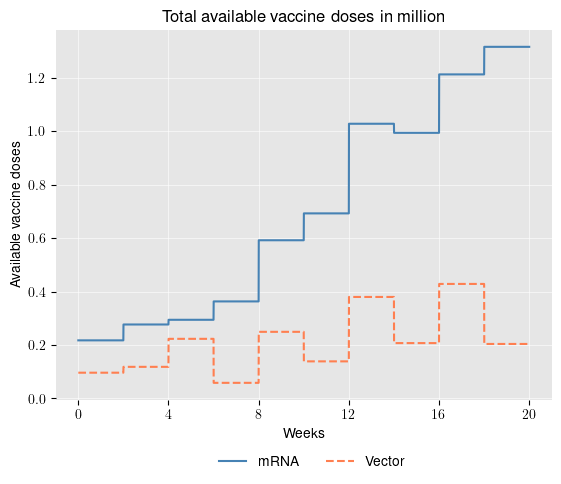
\includegraphics[scale=0.7]{images/available_vaccine.png}\\
\begin{flushleft}
\scriptsize{Note:}
\end{flushleft}
\caption{Vaccines}
\label{fig:available_vaccine}
\end{figure}

\subsection{Simulations}
We use Python and mainly its libraries libSBML \citep{Bornstein.2008} and AMICI \citep{Frohlich.2020} to implement our models. pyPESTO \citep{pyPESTO} is our main tool for optimization. To minimize the optimization problem, we use the L-BFGS-B algorithm \citep{Zhu.1997} for which pyPESTO uses Scipy's \citep{scipy.2020} implementation. For each optimization we run a muli-start using 50 starts and choose the corresponding vaccination strategy that minimizes the objective. For each start, we draw uncorrelated start parameters $\theta_{l,i} \sim \mathcal{U}(0,1)$. In the case of Pareto optimal constraints, we only accept a starting vector $\Theta$ if the Pareto constraints $C.7$ and $C.8$ are satisfied. Otherwise we reject it and draw a new sample until 50 starts are reached.

\textbf{optimal results splines}
fractions in appendix
\begin{figure}[h!]
\centering
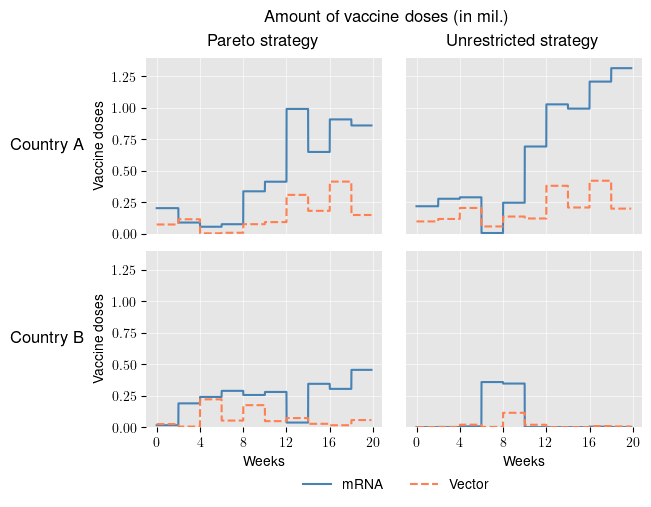
\includegraphics[scale=0.8]{images/piecewise_vaccine_total_quantity.png}\\
\begin{flushleft}
\scriptsize{Note:}
\end{flushleft}
\caption{Vaccines}
\label{fig:results_piecewise_allocation}
\end{figure}

same for infectious individuals
\begin{figure}[h!]
\centering
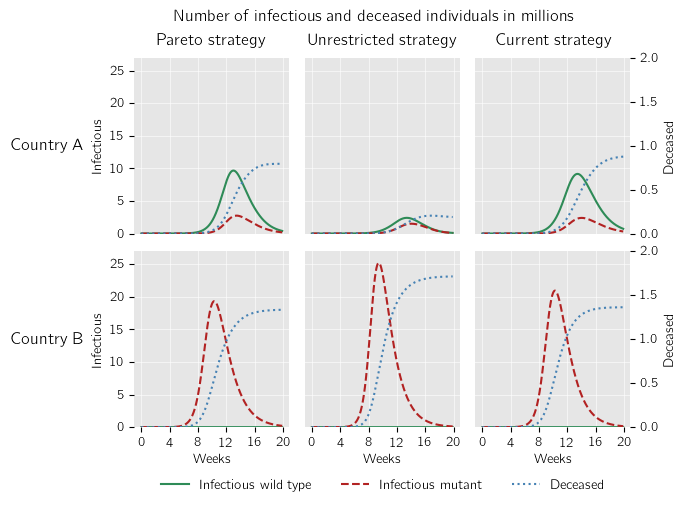
\includegraphics[scale=0.8]{images/piecewise_infectious_dead.png}\\
\begin{flushleft}
\scriptsize{Note:}
\end{flushleft}
\caption{Vaccines}
\label{fig:results_piecewise_infectious_dead}
\end{figure}


waterfall
\begin{figure}[h!]
\centering
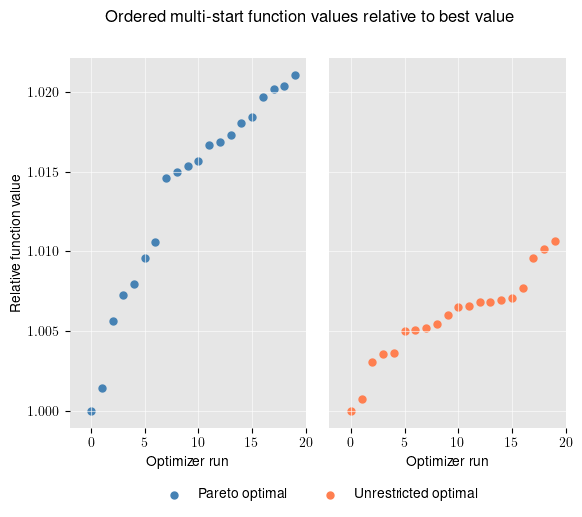
\includegraphics[scale=0.6]{images/piecewise_waterfall.png}\\
\begin{flushleft}
\scriptsize{Note:}
\end{flushleft}
\caption{Vaccines}
\label{fig:results_piecewise_waterfall}
\end{figure}


%\textbf{Optimal results piecewise}
%one plot like in orchestra presentation
%top left, -> total number of assigned, top right fraction, bottom left unvaccinated infectious A; bottom right unvaccinated infectious B;use gs.subplots https://matplotlib.org/devdocs/gallery/subplots_axes_and_figures/subplots_demo.html

same for unrestricted
waterfall plots for both;
4 best strategies for both


table comparing three variants (see orchestra presentation)
{\renewcommand{\arraystretch}{1.4}
\begin{table}[h!]
\centering
\begin{center}
\scalebox{0.8}{
\begin{tabular}{lccp{10cm}}
\hline
\multicolumn{1}{c}{} & \multicolumn{3}{c}{Strategies}\\
\multicolumn{1}{l}{}&\multicolumn{1}{c}{Current}&\multicolumn{1}{c}{Pareto optimal}&\multicolumn{1}{c}{Unrestricted optimal}\\
\hline
\rule{0pt}{2.6ex}Comirnaty & 94\%-95\% &  87\%-95\% &  \cite{Callaway.2021}, \cite{Nasreen.2021}, \cite{Polack.2020}, \cite{Prubeta.2021}, \cite{Sheikh.2021}\\
Spikevax & 94\% &  - & \cite{Oliver.2021}, \cite{Prubeta.2021} \\
Vaxzevria & 66\%-73\% &  60\%-71\% & \cite{Callaway.2021}, \cite{Emary.2021}, \cite{Prubeta.2021}, \cite{Stowe.2021}
 \\
Janssen &  66\% & - & \cite{Oliver.2021a}, \cite{Sadoff.2021} \\
\hline
\end{tabular}
}
\end{center}
\begin{tablenotes}
\scriptsize
\item Note: 
\end{tablenotes}
\caption{Number of deceased individuals depending on the vaccination strategy.}
\label{tab:results_splines}
\end{table}
}



\textbf{optimal results splines}
fractions in appendix
\begin{figure}[h!]
\centering
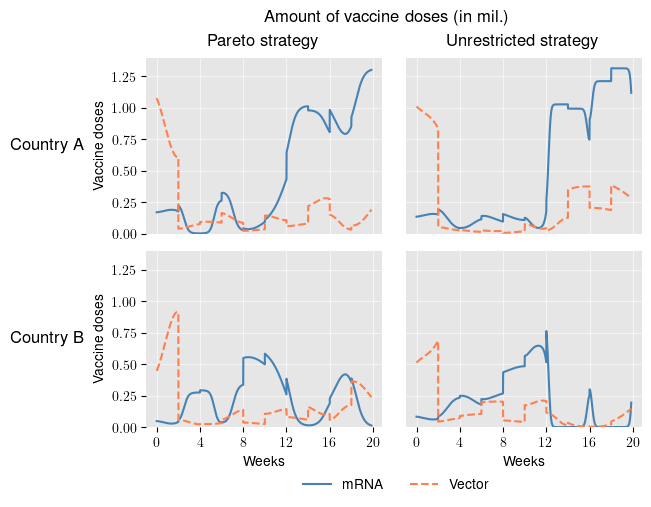
\includegraphics[scale=0.8]{images/splines_vaccine_total_quantity.png}\\
\begin{flushleft}
\scriptsize{Note:}
\end{flushleft}
\caption{Vaccines}
\label{fig:results_splines_allocation}
\end{figure}

same for infectious individuals
\begin{figure}[h!]
\centering
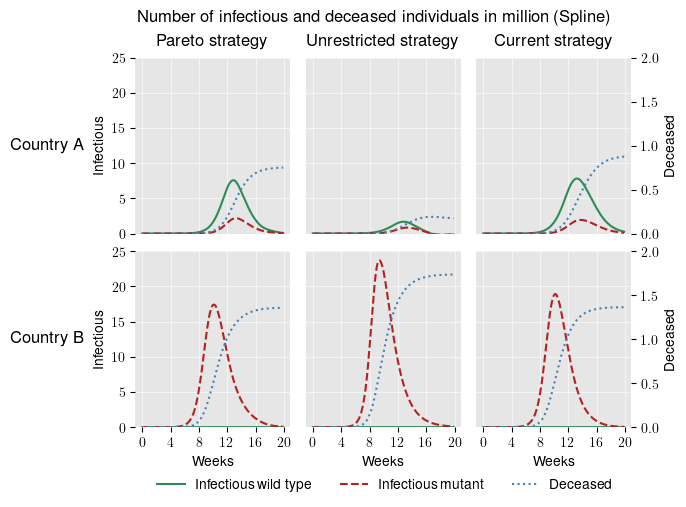
\includegraphics[scale=0.8]{images/splines_infectious_dead.png}\\
\begin{flushleft}
\scriptsize{Note:}
\end{flushleft}
\caption{Vaccines}
\label{fig:results_splines_infectious_dead}
\end{figure}


waterfall
\begin{figure}[h!]
\centering
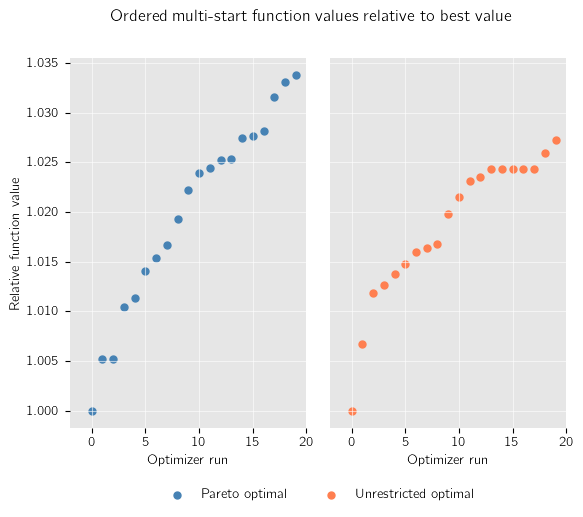
\includegraphics[scale=0.6]{images/splines_waterfall.png}\\
\begin{flushleft}
\scriptsize{Note:}
\end{flushleft}
\caption{Vaccines}
\label{fig:results_splines_waterfall}
\end{figure}

table comparing three variants (see orchestra presentation);

\subsubsection{Test with stochastic set-up}









